\documentclass[hidelinks,11pt]{article}
\usepackage[utf8]{inputenc}
\usepackage{fullpage}
\usepackage{textcomp}
\usepackage{amsmath,amssymb}
\usepackage{setspace}
\usepackage[colorlinks=false]{hyperref}
\usepackage{textcomp} 
\usepackage{fancyhdr}
\usepackage[pdftex]{graphicx}
\usepackage{setspace}
\usepackage{listings}
\usepackage{appendix}
\usepackage[T1]{fontenc}
\usepackage{titlesec}
\usepackage{listings}
\usepackage{color}
\graphicspath{ {./images/} }
\definecolor{gray}{rgb}{.98,.98,.98}
\lstset{frame=tb,
    language=C,                % choose the language of the code
    numbers=left,                   % where to put the line-numbers
    stepnumber=1,                   % the step between two line-numbers.        
    numbersep=5pt,                  % how far the line-numbers are from the code
    backgroundcolor=\color{gray},  % choose the background color. You must add \usepackage{color}
    showspaces=false,               % show spaces adding particular underscores
    showstringspaces=false,         % underline spaces within strings
    showtabs=false,                 % show tabs within strings adding particular underscores
    tabsize=4,                      % sets default tabsize to 2 spaces
    captionpos=b,                   % sets the caption-position to bottom
    breaklines=true,                % sets automatic line breaking
    breakatwhitespace=true,         % sets if automatic breaks should only happen at whitespace
    title=\lstname,
    frame=none,   
    belowskip=0pt,
}
\renewcommand{\headrulewidth}{0pt}
\cfoot{\sc\thepage\ of \pageref{end}}

\begin{document}
\begin{titlepage} % Suppresses displaying the page number on the title page and the subsequent page counts as page 1

	\raggedleft % Right align the title page
	\rule{1pt}{\textheight} % Vertical line
	\hspace{0.05\textwidth} % Whitespace between the vertical line and title page text
	\parbox[b]{0.75\textwidth}{ % Paragraph box for holding the title page text, adjust the width to move the title page left or right on the page
        {\Huge\bfseries Algorithms and\\[0.5\baselineskip]Data Structures }\\[2\baselineskip] % Title
        
        {\large\textit{Notes on Algorithms, Data \\[0.5\baselineskip]Structures and other concepts}}\\[4\baselineskip] % Subtitle or further description
        
        {\Large\textsc{eric li}} % Author name, lower case for consistent small caps
        
        \vspace{0.5\textheight} % Whitespace between the title block and the publisher
        
        %{\noindent The Publisher~~\plogo}\\[\baselineskip] % Publisher and logo
        {\noindent\large\today}\\[\baselineskip]
    }
\end{titlepage}
\tableofcontents
\newpage
\section{Disclaimer}
The author(s) of this document assume(s) no responsibility or liability for any errors or omissions in the content of this document. The information contained in this site is provided on an “as is” basis with no guarantees of completeness, accuracy, usefulness or timeliness or of the results obtained from the use of this information.\\[0.5\baselineskip]
Information provided in this document has been taken from various sources and is by no means a comprehensive record of the source's views nor of the concepts represented.
\section{Trees}
\subsection{Structure}
\subsubsection{Terminology}
Node\\
\section{Linked Lists}
Linked lists are helpful in addressing some of the limitations that arrays face, such as inherent dynamic memory allocation and ease of modification. Instead of memory being assigned for use (as in the programming language C) linked lists are built on the premise of allocating memory as needed, and inserting or deleting as required by the user or data set.
\subsection{Structure}
A linked list is a linear data structure constructed from building blocks called nodes. Like other data structures, a node contains two items: data, which can be simple, compound, pointer, etc. and a memory address reference (or link to the next node). The address reference will access the next node's memory address in the list, and creates a `chain-like' relationship which will naturally produce a linear structure. There are two important nodes that are called the `head node' and the `tail node', which will influence operations and be explained in depth in the following sections.
\begin{figure}[b]
    \centering
    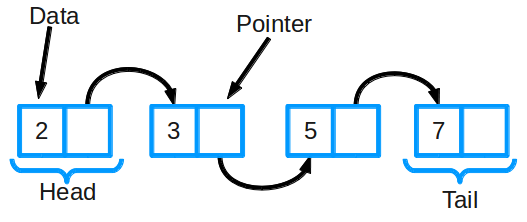
\includegraphics[scale=0.5]{linkedlist.png}
    \caption{Linked List}
\end{figure}
\subsection{Operations}
Linked lists support basic ADT operations of inserting, deleting, and modifying. \\
More specifically, linked lists are constructed by inserting or deleting additional nodes at specified locations in the list. \\
Insertion or deletion at the beginning or end of a list is appropriately named `Head Insertion' and `Tail Insertion' and, `Head Deletion' and `Tail Deletion'.
\\[0.5\baselineskip]
There are two important nodes:
\begin{itemize}
    \item Head Node
    \begin{itemize}
        \item Head insertion is much quicker due to the lack of list traversing done
    \end{itemize}
    \item Tail Node
    \begin{itemize}
        \item Has an address reference of NULL
        \item Entire list must be traversed before tail insertion can occur
    \end{itemize}
\end{itemize}

\subsection{Basic Implementation}
\begin{enumerate}
    \item Define a node
    \begin{lstlisting}
    typedef struct node{
        int num; // data
        struct node *ref; // address
    } node;
    \end{lstlisting}
    \item Dynamic creation of nodes
    \begin{lstlisting}
    node *new_node(void){
        node *p=NULL;
        p=(node *)calloc(1,sizeof(node));
        p->num=0;
        p->ref=NULL;
        return p;
    }
    \end{lstlisting}
\end{enumerate}

\section{Queues}
Queues are built heavily on concepts from linked lists and naturally, follows the same linear data structure. Queues provide a similar environment for "tail insertion" and "head deletion", which are appropriately named "enqueue" and "dequeue" respectively.


\section{Sources}
https://www.cs.cmu.edu/~adamchik/15-121/lectures/Linked%20Lists/linked%20lists.html 
\\
https://medium.com/@kenny.lin/singly-linked-lists-5cfdec60bea0
\end{document}